\documentclass[psamsfonts]{amsart}

%-------Packages---------
\usepackage{amssymb,amsfonts}
\usepackage[all,arc]{xy}
\usepackage{enumerate}
\usepackage{mathrsfs}
\usepackage[margin=1in]{geometry}
\usepackage{thmtools}
\usepackage{verbatim}
\usepackage{multirow}
\usepackage{tikz}
\usetikzlibrary{shapes,arrows}


%--------Theorem Environments--------
%theoremstyle{plain} --- default
\newtheorem{prob}{Problem}[section]
\newtheorem{thm}{Theorem}[section]
\newtheorem{cor}[thm]{Corollary}
\newtheorem{prop}[thm]{Proposition}
\newtheorem{lem}[thm]{Lemma}
\newtheorem{conj}[thm]{Conjecture}
\newtheorem{quest}[thm]{Question}

\newenvironment{sol}{{\bfseries Solution}}{\qedsymbol}


\theoremstyle{definition}
\newtheorem{defn}[thm]{Definition}
\newtheorem{defns}[thm]{Definitions}
\newtheorem{con}[thm]{Construction}
\newtheorem{exmp}[thm]{Example}
\newtheorem{exmps}[thm]{Examples}
\newtheorem{notn}[thm]{Notation}
\newtheorem{notns}[thm]{Notations}
\newtheorem{addm}[thm]{Addendum}
\newtheorem{exer}[thm]{Exercise}

\theoremstyle{remark}
\newtheorem{rem}[thm]{Remark}
\newtheorem{rems}[thm]{Remarks}
\newtheorem{warn}[thm]{Warning}
\newtheorem{sch}[thm]{Scholium}

\makeatletter
\let\c@equation\c@thm
\makeatother
\numberwithin{equation}{section}

\bibliographystyle{plain}

\voffset = -10pt
\headheight = 0pt
\topmargin = -20pt
\textheight = 690pt

%--------Meta Data: Fill in your info------
\title{6.046 \\
Problem Set 3}

\author{John Wang}

\begin{document}

\maketitle

Collaborators: Ryan Liu

\section{Problem A}

\begin{prob}
Describe a simple $O(m^2n)$ time algorithm to solve the electric potential problem. 
\end{prob}

\begin{sol}
The simple algorithm will iterate over all grid points not occupied by a charge, and calculate the sum $\sum_{i=1}^n \frac{q_i}{\sqrt{(x - x_i)^2 + (y - y_i)^2}}$ by iterating over all $n$ grid points with a charge. We will write pseudo-code and then analyze its runtime. First, assume that we have the following input data in matrix form:
\begin{equation}
\left( \begin{array}{c c c}
 q_{11} & \ldots & q_{1m} \\
\vdots & \ddots & \vdots \\
q_{m1} & \ldots & q_{mm}
\end{array} \right)
\end{equation}

Here, $q_{ij} = 0$ if point $(i,j)$ in the grid is not occupied by a charge. Otherwise, $q_{ij}$ denotes the value of the charge at point $(i,j)$ on the gride. Using this input data, the algorithm will have the following pseudocode:

\begin{verbatim}
def find_electric_potential(matrix, m):
    occupied = []
    unoccupied = []
    for i in xrange(m):
        for j in xrange(m):
            if matrix[i][j] != 0:
                occupied.append((i, j, matrix[i][j])
            else:
                unoccupied.append((i,j))

    output = []    
    for (x,y) in unoccupied:
        sum = 0
        for (xi, yi, qi) in occupied:
            sum += qi / ((x - xi)^2 + (y - yi)^2)^(0.5)
        output.append((x, y, sum))
    return output
\end{verbatim}

The algorithm returns the list of tuples: $[(x_1, y_1, V(x_1, y_1)), \ldots, (x_{m-n}, y_{m-n}, V(x_{m-n}, y_{m-n}))]$, where $V(x_i, y_i)$ denotes the potential at $(x_i, y_i)$. The algorithm has a runtime of $O(m^2n)$ because the first block of for loops must iterate over $m^2$ items. The second block of for loops over $m^2 -n$ items, and performs $n$ operations for each of these items. Thus, the total runtime is $O(m^2) + O((m^2-n)n)$. Simplifying this, we obtain: $O(m^2 + m^2n - n^2) = O(m^2n)$ since $m^2 \geq n^2$.    

The correctness of this algorithm follows immediately from the definition of the problem. We compute $V(x_i, y_i)$ exactly as $\sum_{i=1}^n \frac{q_i}{\sqrt{(x - x_i)^2 + (y - y_i)^2}}$ for each of the unoccupied points. 
\end{sol}

\section{Problem B}

\begin{prob}
Let $\mathrm{Z}_{2m-1}={0,1,\ldots,2m-2}$.  Find two functions
$f,g:\mathrm{Z}_{2m-1}\times \mathrm{Z}_{2m-1} \to \mathrm{R}$ such that the
potential at $(x,y)$ for $0 \leq x,y < m$ equals the convolution of $f$ and $g$:
\begin{eqnarray*}
V(x,y) & = & (f\otimes g)(x,y) \\
& = & \sum_{x'=0}^{2m-2}\sum_{y'=0}^{2m-2} f(x',y')\cdot
g(x-x',y-y')\ .
\end{eqnarray*}
Importantly, in this definition $x-x'$ and $y-y'$ are computed in the
additive group $\mathrm{Z}_{2m-1}$, which is a fancy way of saying
they are computed modulo $2m-1$.
\end{prob}

\begin{sol}
We shall take the following functions:
\begin{equation}
f(x,y) = \left\{ \begin{array}{c c}
0 & \text{if } x > m-1 \text{ or } y > m- 1 \\
\frac{q(x,y)}{4 \pi \epsilon_0} & \text{otherwise}
\end{array} 
\right.
\end{equation}

And also we take:
\begin{equation}
g(x,y) = \left\{ \begin{array}{c c} 
0 & \text{if } x =0, y = 0 \\
(\bar{x}^2 + \bar{y}^2)^{-1/2} & \text{otherwise}
\end{array} \right.
\end{equation}

Where $\bar{x}$ and $\bar{y}$ are defined as follows:
\begin{equation}
\begin{array}{c c}
\bar{x} = \left\{ \begin{array}{c c} 
x & \text{if } x < m \\
2m - 1 - x & \text{if } x \geq m 
\end{array} \right.
& 
\bar{y} = \left\{ \begin{array}{c c} 
y & \text{if } y < m \\
2m - 1 - y & \text{if } y \geq m 
\end{array} \right.
\end{array}
\end{equation}

We know that $x - x'$ ranges from $-(m-1)$ to $(m-1)$. However, we know that $- (m - 1) \equiv -(m - 1) + 2m - 1 \equiv m \pmod{2m - 1}$. Thus, if $x - x' > m$, all we need to do is subtract $x$ from $2m - 1$ to obtain a correct mapping. The same can be done for $y - y'$.  

We shall show that these two functions satisfy $V(x,y) = (f \otimes g)(x,y)$. This can be shown by simply expanding the definitions. We know the following:
\begin{eqnarray}
(f \otimes g)(x,y) &=& \sum_{x'=0}^{2m-2} \sum_{y'=0}^{2m-2} f(x',y') g(x - x', y - y') \\
&=& \sum_{x'=0}^{m-1} \sum_{y'=0}^{m-1} \frac{q(x',y')}{4 \pi \epsilon_0} g(x -x', y-y') \\
&=& \sum_{x'=0}^{m-1} \sum_{y'=0}^{m-1} \frac{q(x',y')}{4 \pi \epsilon_0} \frac{1}{\sqrt{(x-x')^2 + (y - y')^2}} \\
&=& \sum_{i=1}^{n} \frac{ q_i}{4 \pi \epsilon_0 \sqrt{ (x-x_i)^2 + (y - y_i)^2}} \\
&=& V(x,y)
\end{eqnarray}

Where the last part follows since $q(x',y') = 0$ unless it holds a charge $q_i$. Thus, we have choosen functions $f$ and $g$ which satisfy the property that their convolutions lead to the electric potential.
\end{sol}

\section{Problem C}

\begin{prob}
Prove that for any two
functions $f,g:\mathrm{Z}_{k}\times \mathrm{Z}_{k} \to \mathrm{R}$ and for any
point $(a,b)\in \mathrm{Z}_{k}\times \mathrm{Z}_{k}$, we have
\[
\widehat{(f\otimes g)}(a,b) = k^2\cdot\widehat{f}(a,b)\cdot\widehat{g}(a,b)\ .
\]
\end{prob}

\begin{sol}
First, we shall expand $k^2 \widehat{f}(a,b) \cdot \widehat{g}(a,b)$ using the definition of the discrete fourier transform:
\begin{eqnarray}
k^2\cdot\widehat{f}(a,b)\cdot\widehat{g}(a,b) &=& \frac{1}{k^2} \left( \sum_{x=0}^{k-1} \sum_{y=0}^{k-1} f(x,y) w_k^{-ax-by} \right) \left( \sum_{x'=0}^{k-1} \sum_{y'=0}^{k-1} g(x',y') w_k^{-ax'-by'} \right) \\
&=& \frac{1}{k^2} \sum_{x=0}^{k-1} \sum_{y=0}^{k-1} \sum_{x' = 0}^{k-1} \sum_{y' = 0}^{k-1} f(x,y) g(x',y') w_k^{-a(x+x') - b(y + y')}
\end{eqnarray}

Now, we want to see what $\widehat{(f\otimes g)}(a,b)$ is equal to. We shall expand this expression according to the definitions of convolution and discrete fourier transforms:
\begin{eqnarray}
\widehat{(f\otimes g)}(a,b) &=& \frac{1}{k^2} \sum_{x=0}^{k-1} \sum_{y=0}^{k-1} \widehat{(f\otimes g)}(x,y) w_k^{-ax - by} \\
&=& \frac{1}{k^2} \sum_{x=0}^{k-1} \sum_{y=0}^{k-1} \left( \sum_{x'=0}^{k-1} \sum_{y'=0}^{k-1} f(x',y') g(x-x', y-y') \right) w_k^{-ax-by} 
\end{eqnarray}

Notice that the sum inside the parentheses can be broken up into two sums. The first group shall consist of $x,x',y,y'$ combinations such that $x - x' > 0$, $x - x' < k-1$, $y - y' > 0$, and $y - y' < k -1$. The second group shall consist of $x,x',y,y'$ combinations such that $x - x' < 0$, $x- x' > -(k - 1)$, $y - y' < 0$, and $y - y' > -( k -1)$. However, since $x - x'$ and $y -y'$ are taken modulo $k -1$, we see that these two groups yield the same sums. Writing this out, we have:
\begin{eqnarray}
&=& \frac{1}{k^2} \sum_{x=0}^{k-1} \sum_{y=0}^{k-1} \left( \sum_{x'=x - (k - 1)}^{x} \sum_{y' = y - (k -1)}^{y} f(x',y') g(x - x', y -y') \right. \\
&+& \left. \sum_{x' = x}^{x + (k -1)} \sum_{y' = y}^{y + (k -1)} f(x',y') g(x-x', y-y') \right) w_k^{-ax-by}
\end{eqnarray}  

Since the set $\{0, 1, \ldots k-1\}$ is congruent to $\{-(k-1), -(k-1)+1, \ldots, -1\}$ modulo $k-1$, we see that the sums in between the parentheses in the above equation can be combined into:
\begin{eqnarray}
&=& \frac{1}{k^2} \sum_{x=0}^{k-1} \sum_{y=0}^{k-1} \sum_{\bar{x}=0}^{k-1} \sum_{\bar{y} = 0}^{k-1} f(x',y') g(\bar{x},\bar{y}) w_k^{-a(\bar{x} + x') - y (\bar{y} + y') } 
\end{eqnarray} 

Where we have made the transformation $\bar{x} = x - x'$ and $\bar{y} = y - y'$. Looking back at our expanded expresion of $k^2 \widehat{f}(a,b) \cdot \widehat{g}(a,b)$, it is clear that we have shown $\widehat{(f\otimes g)}(a,b) = k^2\cdot\widehat{f}(a,b)\cdot\widehat{g}(a,b)$ to be true.
\end{sol}

\section{Problem D}

\begin{prob}
Design an $O(k^2 \lg k)$ time algorithm to compute the discrete Fourier transform and its
inverse.
\end{prob}

\begin{sol}
For a function $h(x,y): \mathrm{Z}_{k} \times \mathrm{Z}_{k} \to \mathrm{C}$, we would like to compute the discrete Fourier transform defined as the following:
\begin{eqnarray}
\widehat{h}(a,b) &=& \frac{1}{k^2} \sum_{x=0}^{k-1} \sum_{y=0}^{k-1} h(x,y) w_k^{-ax-by} \\
&=& \frac{1}{k^2} \sum_{x=0}^{k/2 - 1} \sum_{y=0}^{k/2 - 1}  \left( h(2x, 2y) w_k^{-2ax - 2by} + h(2x + 1, 2y + 1) w_k^{-a(2x + 1) - b(2y + 1)} \right. \\
& & + \left. h(2x, 2y+1) w_k^{-2ax - b(2y+1)} + h(2x+1,2h) w_k^{-a(2x+1) - 2y} \right) \nonumber \\
&=& \frac{1}{k^2} \sum_{x=0}^{k/2 - 1} \sum_{y=0}^{k/2 - 1} h(2x, 2y) w_{k/2}^{-ax - by} +  \frac{w_{k}^{-a - b}}{k^2} \sum_{x=0}^{k/2 - 1} \sum_{y=0}^{k/2 - 1}  h(2x + 1, 2y + 1) w_{k/2}^{-ax -by}   \\
& & + \frac{w_k^{-b}}{k^2} \sum_{x=0}^{k/2-1} \sum_{y=0}^{k/2-1} h(2x+1, 2y) w_{k/2}^{-ax - by} + \frac{w_k^{-a}}{k^2} \sum_{x=0}^{k/2-1} \sum_{y=0}^{k/2 - 1} h(2x, 2y+1) w_{k/2}^{-ax-by} \nonumber
\end{eqnarray} 

The last equation comes from the fact that $w_k^2 = w_{k/2}$. We have split the problem up into finding the discrete Fourier transform for $h(a,b)$ where $a,b$ are even, $a,b$ are odd, and $a,b$ are alternating even and odd. However, we have decreased our space by half, so that we are left with much less work. 

The only difference is that there is a sign change in the last expression to accomodate the fact that $a$ and $b$ are in $\{k/2, \ldots, k-1 \}$. Using this as the mathematical background of our algorithm, we can now develop an $O(k^2 \lg k)$ time algorithm for computing the discrete fourier transform. Since we want to compute $\widehat{h}(a,b)$, and we have shown that $\widehat{h}(a,b)$ can be broken apart into two smaller problems, we can use a recursive, divide and conquer approach. The pseudo-code is given below:

\begin{verbatim}
def dft(q, k):
    if k = 1:
        return q[0][0]
    else:
        Initiate Q as a k by k output matrix 
        out1 = dft(q[x][y] where x,y are even, k/2)
        out2 = dft(q[x][y] where x,y are odd, k/2)
        out3 = dft(q[x][y] where x is even and y is odd, k/2)
        out4 = dft(q[x][y] where x is odd and y is even, k/2)
        for x in xrange(k/2-1):
            for y in xrange(k/2-1):
                Q[x][y] = (out1[x][y] + out2[x][y]*unityroots(k,-a-b)
                        + out3[x][y]*unityroots(k,-b)
                        + out4[x][y]*unityroots(k,-a))/k^2 
                Q[x+k/2][y+k/2] = Q[x][y]
        return Q
\end{verbatim}

The inverse can be computed similarly, but by dropping the $\frac{1}{k^2}$ term. The code for the inverse is so close to the code for the dft function that we will not write it again. Moreover, it is clear that by changing the multiplicative term, we do not change the runtime. 

For an analysis of the runtime, we start with a problem of size $k$. In the algorithm, we run $dft(q, k/2)$ four times, then we perform $O(k^2)$ arithmetic operations (we will say that addition, multiplication, and division all take $O(1)$). Then, we have the recurrence:
\begin{eqnarray}
T(k) &=& 4T(k/2) + ck^2 \\
&=& ck^2 + 4(c(k/2)^2 + 4T(k/4)) \\
&=& ck^2 + ck^2 + 16(c(k/4)^2 + T(k/8)^2 \\
&=& \underbrace{ck^2 + \ldots + ck^2}_{\lg k} \\
&=& c k^2 \lg k
\end{eqnarray}

Therefore, the running time is $T(k) = O(k^2 \lg k)$, which is what we wanted. We have already shown correctness since we are using equation (4.2) to compute $\widehat{h}(a,b)$ in our algorithm. We have only rearranged terms in $\widehat{h}(a,b)$ and used the fact that $w_k^2 = w_{k/2}$ to design our algorithm. The proof of correctness follows from equation $(4.2)$, assuming that $k$ is a power of 2. 

The diagram below shows the intricacies of the algorithm. Computing the discrete Fourier transform involves breaking it apart into four smaller pieces. These consist of indices $i,j$ such that they are even/even, even/odd, odd/even, and odd/odd. The diagram below shows how one would split up a $4 \times 4$ matrix into different subproblems. 

\begin{figure}[h!]
\centering
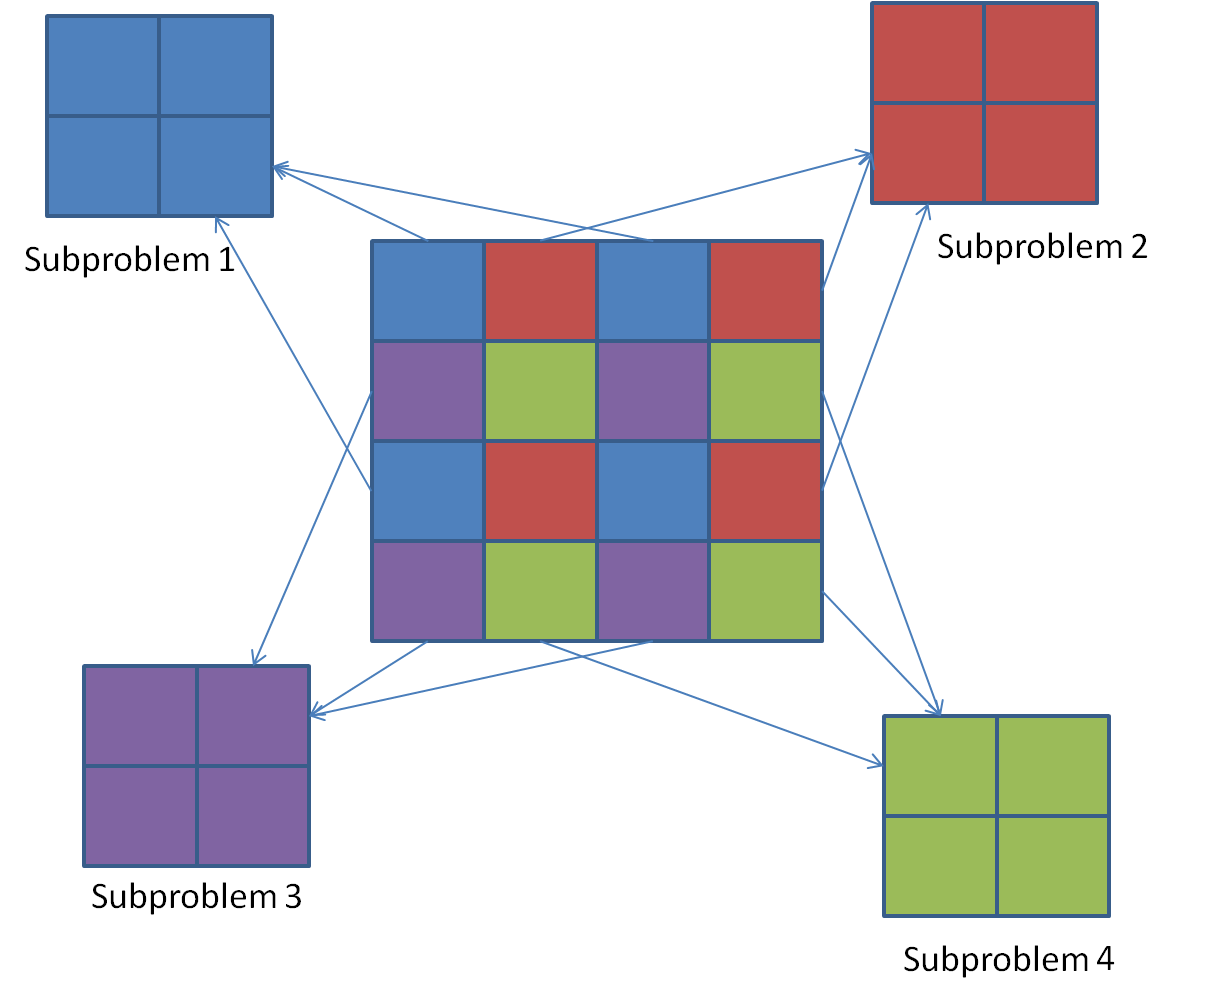
\includegraphics[width=3in]{diagram.png}
\caption{Diagram of Subproblem Partitioning}
\end{figure}
\end{sol}

\section{Part E}

\begin{prob}
Design an $O(m^2 \lg m)$ time algorithm to soilve the electric potential problem for a grid of size $m \times m$. 
\end{prob}

\begin{sol}
\begin{figure}[h!]
\centering
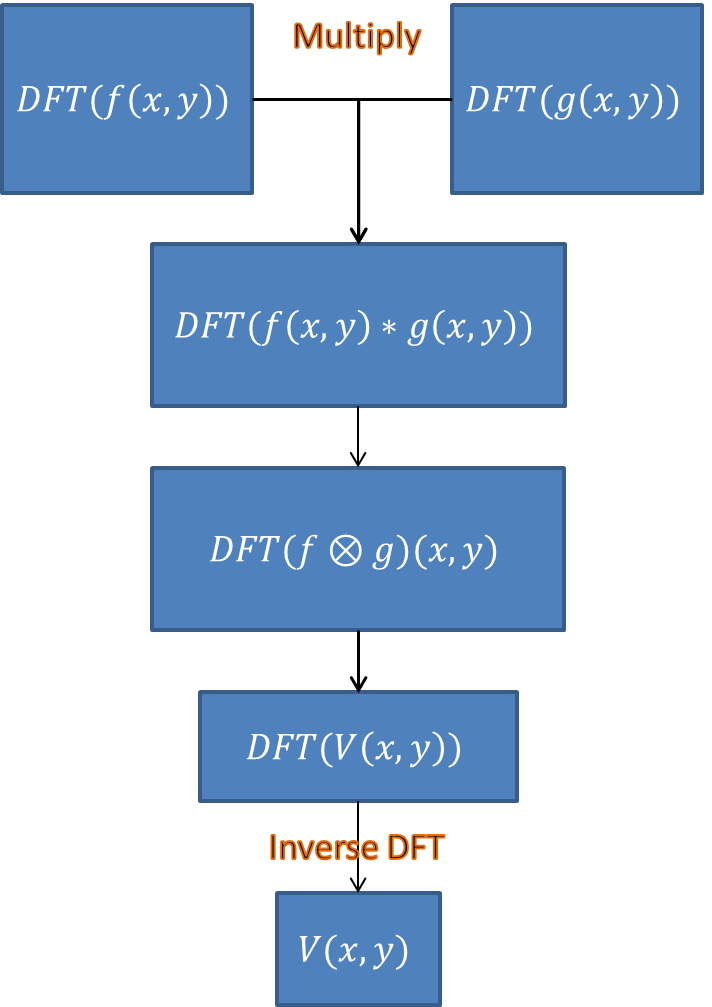
\includegraphics[width=2.3in]{FlowChart.png}
\caption{Flow Chart of the Algorithm}
\label{flow}
\end{figure}

We will use the $O(k^2 \lg k)$ algorithm to compute the discrete Fourier transform and the two functions $f$ and $g$ defined in part $b$ to complete this algorithm. First, we know that $V(x,y) = (f \otimes g) (x,y)$. Moreover, we know that $\widehat{(f \otimes g)}(x,y) = \widehat{f}(x,y) \widehat{g}(x,y)$ by part $c$. Thus, we know that $\widehat{V}(x,y) =  \widehat{f}(x,y) \widehat{g}(x,y)$. Thus, in order to find $V(x,y)$, we can simply take the inverse discrete Fourier transform of $\widehat{f} \widehat{g}$. Denote the inverse discrete Fourier transform of a function $f$ by $dft^{-1}(f)$. We know the following:
\begin{eqnarray}
V(x,y) = dft^{-1}(\widehat{f}(x,y) \widehat{g}(x,y))
\end{eqnarray}

However, we already have an algorithm that computes $\hat{f}(x,y)$ and $\hat{g}(x,y)$ in $O(k^2 \lg k)$, where $k$ is size of the $k \times k$ space. However, since $f,g : \mathrm{Z}_{m} \times \mathrm{Z}_m \to \mathrm{C}$, we see that $k = m$ and the algorithm runs in $O(m^2 \lg m)$. Moreover, we can compute $dft^{-1} (\widehat{f}(x,y) \widehat{g}(x,y) )$ in $O(m^2 \lg m)$ because the inverse discrete Fourier transform takes the same time as the discrete Fourier transform, and multiplication takes $O(1)$ time. Therefore, we see that we can compute $V(x,y)$ in a total time of $O(m^2 \lg m)$. 

The algorithm, then, is as follows: take the discrete Fourier transform of $f(x,y)$ ad $g(x,y)$ as defined in part $b$ on the space $\mathrm{Z}_m \times \mathrm{Z}_k$. Then, multiply the together, and take the inverse discrete Fourier transform of the product. This should give the electric potential at all points $(x,y)$ where $x,y \in \{0, \ldots, m-1\}$. To finish the problem, we return the potentials at the points $(x_i, y_i)$ which are not occupied by a charge. 

The correctness of this algorithm follows from the argument given in the first paragraph. It relies on the observations pointed out in parts $b,c,$ and $d$. A diagram/example of the algorithm is given in the figure \ref{flow}.

\end{sol}

\end{document}